\documentclass[pdflatex,compress,mathserif]{beamer}

%\usetheme[dark,framenumber,totalframenumber]{ElektroITK}
\usetheme[darktitle,framenumber,totalframenumber]{ElektroITK}

\usepackage[utf8]{inputenc}
\usepackage[T1]{fontenc}
\usepackage{lmodern}
\usepackage[bahasai]{babel}
\usepackage{amsmath}
\usepackage{amsfonts}
\usepackage{amssymb}
\usepackage{graphicx}
\usepackage{multicol}
\usepackage{lipsum}

\newcommand*{\Scale}[2][4]{\scalebox{#1}{$#2$}}%

\title{METODE NUMERIK}
\subtitle{Interpolasi Polinom}

\author{Tim Dosen Pengampu}

\begin{document}

\maketitle

\section{Pengantar}

\begin{frame}
	\frametitle{Pengantar}
	\begin{itemize}
		\item Sebuah pengukuran fisika telah dilakukan untuk menentukan hubungan antara tegangan yang diberikan kepada baja tahan-karat dan waktu yang diperlukan hingga baja tersebut patah.
		\item Delapan nilai tegangan yang berbeda dicobakan, dan data yang dihasilkan adalah
		\begin{center}
			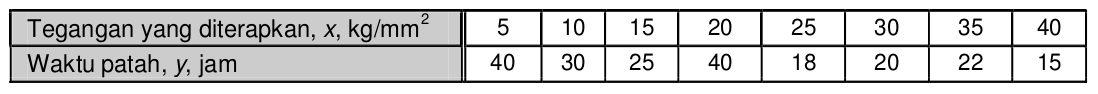
\includegraphics[width=\linewidth]{img/img01}
		\end{center}
		\item Berapa waktu patah $ y $ jika tegangan $ x $ yang diberikan kepada baja adalah 12 kg/mm$ ^2 $ .
	\end{itemize}
\end{frame}

\begin{frame}
	\begin{itemize}
		\item Solusinya dicari dengan metode pencocokan kurva (\textit{curve fitting}).
		\item Yaitu mencari fungsi yang mencocokkan (\textit{fit}) titik-titik data di dalam tabel tabel.
		\item Pencocokkan kurva adalah sebuah metode yang mencocokkan titik data dengan sebuah kurva (\textit{curve fitting}) fungsi.
		\item Pencocokan kurva dibedakan atas dua metode:
		\begin{enumerate}
			\item Regresi
			\item Interpolasi
		\end{enumerate}
	\end{itemize}
\end{frame}

\begin{frame}
	\begin{enumerate}
		\item \textbf{Regresi}
		\begin{itemize}
			\item Data hasil pengukuran umumnya mengandung derau (\textit{noise}) atau galat yang cukup berarti.
			\item Karena data ini tidak teliti, maka kurva yang mencocokkan titik data itu tidak perlu melalui semua titik.
			Kurva tersebut cukup hanya mewakili kecenderungan (\textit{trend}) titik data, yakni kurva mengikuti pola titik sebagai suatu kelompok.
		\end{itemize}
	\end{enumerate}
\end{frame}

\begin{frame}
	\begin{enumerate}
		\setcounter{enumi}{1}
		\item \textbf{Interpolasi}
		\begin{itemize}
			\item Bila data diketahui mempunyai ketelitian yang sangat tinggi, maka kurva cocokannya dibuat melalui setiap titik.
			\item Kita katakan di sini bahwa kita \textbf{menginterpolasi} titik-titik data dengan sebuah fungsi.
			\item Bila fungsi cocokan yang digunakan berbentuk polinom, polinom tersebut dinamakan \textbf{polinom interpolasi}.
			\item Pekerjaan menginterpolasi titik data dengan sebuah polinom disebut \textbf{interpolasi (dengan) polinom}.
		\end{itemize}
	\end{enumerate}
\end{frame}

\begin{frame}
	\begin{center}
		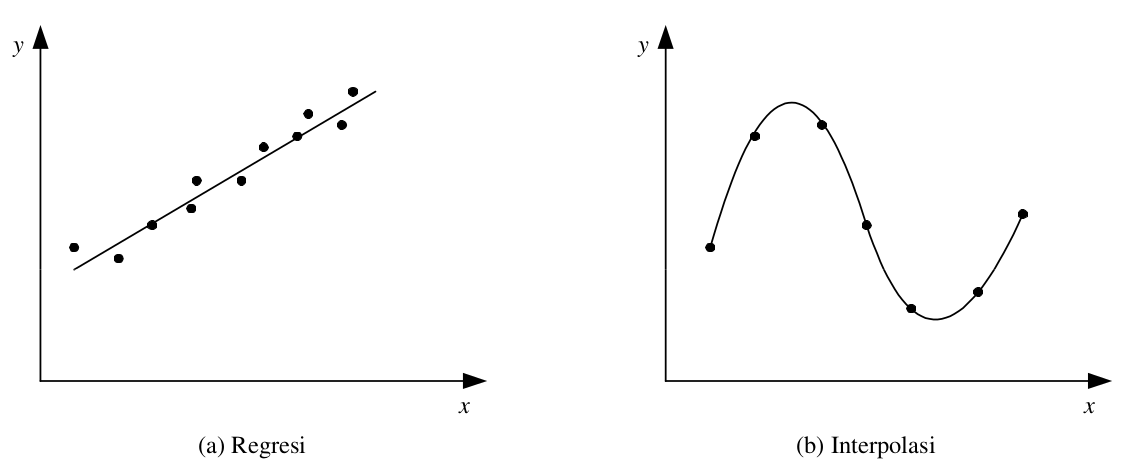
\includegraphics[width=\linewidth]{img/img02}
	\end{center}
\end{frame}

\begin{frame}
	\frametitle{Aplikasi Interpolasi Polinom}
	\begin{enumerate}
		\item Menghampiri fungsi rumit menjadi lebih sederhana
		\begin{itemize}
			\item Contoh: \[ f(x) = \frac{\ln(2x^{(1/2)}-4x^2)^3}{\sqrt{1+2x^5}} \]
			\item[] Hitung: $ f'(x) $ dan $\int f(x) dx$
			\item Perhitungan menjadi lebih mudah jika $ f(x) $ dihampiri dengan polinom $ p(x) $.
			\item Polinom $ p(x) $ diperoleh dengan menginterpolasi beberapa titik diskrit dari $ f(x) $
		\end{itemize}
		\item Menggambar kurva (jika hanya diketahui titik-titik diskrit saja)
	\end{enumerate}
\end{frame}

\section{Interpolasi Polinom}

\begin{frame}
	\frametitle{Interpolasi Polinom}
	\textbf{Persoalan}
	\begin{itemize}
		\item Diberikan $ n+1 $ buah titik berbeda, ($ x_0 $, $ y_0 $ ), ($ x_1 $, $ y_1 $ ), $\dots$, ($ x_n $ , $ y_n $ ).
		\item Tentukan polinom $ p_n(x) $ yang menginterpolasi (melewati) semua titik-titik tersebut sedemikian rupa sehingga
		\[ y_i = p_n(x_i)\qquad \text{ untuk } i = 0,1,2,\dots,n \]
		\item Nilai $ y_i $ dapat berasal dari fungsi $ f(x) $ sedemikian sehingga \[ y_i = f(x_i), \] atau, $ y_i $ berasal dari nilai empiris yang diperoleh melalui percobaan atau pengamatan.
	\end{itemize}
\end{frame}

\begin{frame}
	\begin{itemize}
		\item $ p_n(x) $ disebut fungsi hampiran terhadap $ f(x) $.
		\item Setelah polinom interpolasi $ p_n(x) $ ditemukan, $ p_n(x) $ dapat digunakan untuk menghitung perkiraan nilai $ y $ di $ x = a $, yaitu $ y = p_n(a) $.
		\item Bergantung pada letaknya, nilai $ x = a $ mungkin terletak di dalam rentang titik-titik data ($ x_0 < a < x_n $ ) atau di luar rentang titik-titik data ($ a < x_0 $ atau $ a > x_n $ ):
		\begin{enumerate}
			\item jika $ x_0 < a < x_n $ maka $ y_k = p(x_k) $ disebut \textbf{nilai interpolasi} (\textit{interpolated value})
			\item jika $ x_0 < x_k $ atau $ x_0 < x_n $ maka $ y_k = p(x_k) $ disebut nilai \textbf{ekstrapolasi} (\textit{extrapolated value}).
		\end{enumerate}
	\end{itemize}
\end{frame}

\begin{frame}
	\begin{center}
		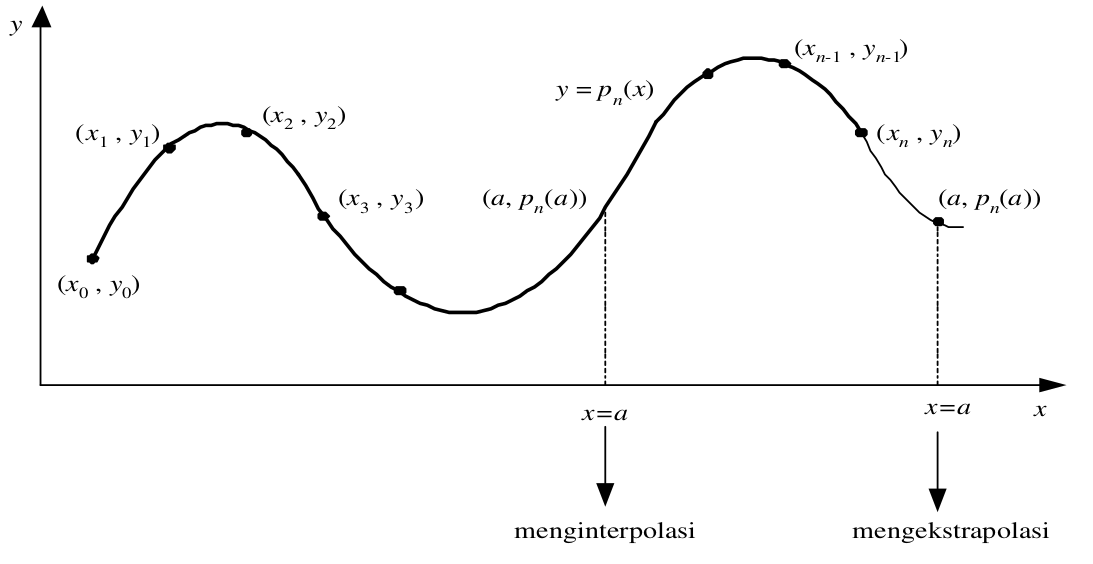
\includegraphics[width=0.7\linewidth]{img/img03}
	\end{center}
	\begin{itemize}
		\item Kita dapat menginterpolasi titik data dengan: polinom lanjar, polinom kuadratik, polinom kubik, atau polinom dari derajat yang lebih tinggi, bergantung pada jumlah titik data yang tersedia.
	\end{itemize}
\end{frame}

\subsection{Interpolasi Lanjar}

\begin{frame}
	\frametitle{Interpolasi Lanjar}
	\begin{itemize}
		\item Interpolasi lanjar adalah interpolasi dua buah titik dengan sebuah garis lurus.
		\item Misal diberikan dua buah titik, $ (x_0 , y_0) $ dan $ (x_1, y_1) $. Polinom yang menginterpolasi kedua titik itu adalah \[ p_1 (x) = a_0 + a_1 x \]
	\end{itemize}
	\begin{multicols}{2}
		\[ y_0 = a_0 + a_1 x_0;~y_1 = a_0 + a_1 x_1 \] menjadi
		\[ a_1 = \frac{y_1 - y_0}{x_1 - x_0};~a_0 = \frac{x_1 y_0 - x_0 y_1}{x_1 - x_0} \] sehingga
		\[ p_1(x) = \frac{x_1 y_0 - x_0 y_1}{x_1 - x_0} +  \frac{y_1 - y_0}{x_1 - x_0} x \]
		\columnbreak
		\begin{center}
			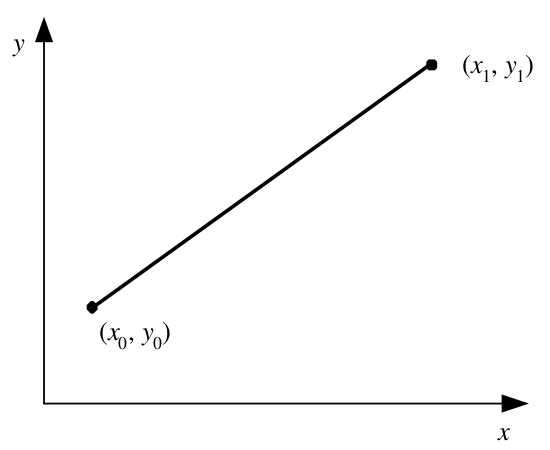
\includegraphics[width=0.8\linewidth]{img/img04}
		\end{center}
	\end{multicols}
\end{frame}

\end{document}
